\documentclass[serif, xcolor={svgnames, table}, usepdftitle=false]{beamer}

% Beamer
\usetheme{Madrid}
% \usecolortheme{beaver}
\usefonttheme{professionalfonts}
\beamertemplatenavigationsymbolsempty

% Fonts
\usepackage{fontspec}

% Languages and bibliographies
\usepackage{polyglossia}
\usepackage{csquotes}
\usepackage[hyperref, backend=biber, maxnames=3, minnames=1,
isbn=false, url=false, doi=false, eprint=false]{biblatex}

% Mathematics
\usepackage{mathtools}
\usepackage{amsthm}
\usepackage[math-style=TeX, bold-style=upright]{unicode-math}

% Pseudocode
\usepackage{algorithm}
\usepackage{algpseudocode}
\usepackage{varwidth}

% Proofs
\usepackage{prftree}

% Source code
\usepackage[newfloat]{minted}

% Microtype
\usepackage[babel]{microtype}

% Graphics and captioning
\usepackage{graphicx}
\usepackage[compatibility=false]{caption}
\usepackage{subcaption}

% Tables
\usepackage{booktabs}

% Frames
\usepackage[framemethod=tikz]{mdframed}

% Numbers
\usepackage{siunitx}
\usepackage{nth}

% Cryptography (load after `hyperref`)
\usepackage[n, advantage, operators, sets, adversary,
landau, probability, notions, logic, ff, mm, primitives,
events, complexity, asymptotics, keys]{cryptocode}

% Dashes and hyphens (load at the end)
\usepackage[shortcuts]{extdash}

%
% Package setup
%

\setmainlanguage{english}
\setmathfont{Latin Modern Math}
\mathtoolsset{mathic=true}
\sisetup{%
  detect-all,
  detect-display-math,
  binary-units
}

\graphicspath{{Figures/}{../}}

\addbibresource{Bibliography.bib}
\DeclareFieldFormat{url}{\texttt{\url{#1}}}
\renewcommand*{\bibfont}{\small}

\hypersetup{%
  unicode,
  breaklinks,
  pdfinfo={%
    Title={Recent Topics in Compilers and Programming Languages},
    Subject={Compilers and Programming Languages},
    Author={Dario Gjorgjevski and Petar Tonkovikj},
    Keywords={Compilers, Programming Languages, Dependent Types,
      Automatic Vectorization, Automatic Parallelization}
  }
}

\AtBeginDocument{%
  % Vectors and matrices
  \renewcommand*{\vec}[1]{\symbf{#1}}
  \newcommand{\mat}[1]{\symbf{#1}}
  \newcommand{\trans}{\intercal}

  % Operators
  \DeclareMathOperator{\rank}{rank}
  \DeclareMathOperator*{\argmin}{arg\,min}
  \DeclareMathOperator*{\argmax}{arg\,max}
}

% Custom operators
\DeclareMathOperator{\valid}{valid}

%
% Title
%

\title[Recent Topics in Compilers]{Recent Topics in Compilers and Programming Languages}
\subtitle{Dependent Types and Automatic Vectorization and Parallelization}
\author[D.~Gj. and P.~T.]{%
  Dario Gjorgjevski\inst{1} \and Petar Tonkovikj\inst{1}\\%
  {\ttfamily\{\href{mailto:gjorgjevski.dario@students.finki.ukim.mk}{gjorgjevski.dario},\href{mailto:tonkovikj.petar@students.finki.ukim.mk}{tonkovikj.petar}\}@students.finki.ukim.mk}
}
\institute[FCSE]{%
  \inst{1}Faculty of Computer Science and Engineering\\%
  Ss.\ Cyril and Methodius University in Skopje
}
\date{\today}

%
% Table of contents
%

\AtBeginSection[]{%
  \begin{frame}{Contents}
    \tableofcontents[currentsection]
  \end{frame}
}

%
% Document
%

\begin{document}
\begin{frame}
  \titlepage
\end{frame}

\section{Introduction}

\begin{frame}{Compilers}{Not so modern, even today?}
  Even today, the architecture of a compiler is the same as it was
  more than thirty years ago, when the modern foundations were laid
  out.  Nonetheless, that is only the big picture -- the difference is
  in the little things:
  \begin{itemize}
  \item Functional languages are gaining traction.  Type theory and
    \(\lambda\)-calculi are being researched more than ever.
  \item Compilers are becoming smarter:
    \begin{itemize}
    \item JIT and dynamic optimizations are extended to static
      languages.
    \item Compilers help in tackling multi-core programming.
    \item Compilers are (partially) responsible for memory safety.
    \end{itemize}
  \end{itemize}
\end{frame}

\begin{frame}{Today's topics}
  We have researched two topics: one related to functional programming
  and type theory, and the other to code optimization.
  \begin{description}
  \item[Dependent types] Types whose definition depends on a value.
  \item[Exploiting parallelism] Automatic vectorization and
    parallelization.
  \end{description}

  We believe that these topics are very relevant to today's trends in
  compilers and programming languages, and will try to introduce you
  to them.
\end{frame}

\section{Dependent types}
\begin{frame}{Dependent types}{Motivation}
  Types matter.  They allow us to classify data:
  \begin{itemize}
  \item how to store them in memory;
  \item whether they can safely be passed to an operation; and
  \item who is allowed to see them.
  \end{itemize}

  Dependent types are expressed in terms of data, explicitly relating
  their inhabitants to the data.
\end{frame}

\begin{frame}[fragile]{Dependent types}{Motivating example}
  Consider the typical \mintinline{haskell}{head} function.
  \begin{minted}{haskell}
    head :: a list -> a
    head (x : xs) = x
    head [] = error "no head"
  \end{minted}

  \begin{alertblock}{Program correctness}
    Is \mintinline{haskell}{head z} a correct program?  A traditional
    (e.g., Haskell's) type checker can't tell.
  \end{alertblock}
\end{frame}

\begin{frame}[fragile]{Dependent types}{Fixing things}
  Let us create a datatype that tracks the length at compile-time.
  \begin{minted}[autogobble, escapeinside=!!]{haskell}
    data Nat = 0 | Succ Nat
    data Vec (a : *) (n : Nat) where
      nil  : Vec a 0
      cons : a -> Vec a n -> Vec a (Succ n)

    head :: !$\Pi$! (x : Nat). Vec a (Succ x) -> a
    head (cons x xs) = x
    -- head nil case is impossible!
  \end{minted}

  \begin{block}{Success!}
    If \mintinline{haskell}{head z} typechecks, it must be correct,
    i.e., there must be a head.
  \end{block}
\end{frame}

\begin{frame}{Formal definition}
  \begin{definition}[Dependent type]\label{def:dependent-type}
    Given a type \(A : \mathcal{U}\) in a universe of types
    \(\mathcal{U}\), let \(B \colon A \to \mathcal{U}\) be a
    \emph{family of types} which assigns to each term \(x : A\) a type
    \(B(x) : \mathcal{U}\).

    A function whose type of return value varies with its argument
    (i.e., it has no fixed codomain) is called a \emph{dependent
      type}.  It is written as
    \[
      \prod\limits_{(x : A)} B(x)\text{.}
    \]
  \end{definition}

  A ``pair of integers'' is a type.  A ``pair of integers where the
  second is greater than the first'' is a dependent type because of
  the dependence on the value.
\end{frame}

\begin{frame}[fragile]{More applications}{Attaching invariants to
    datatypes}
  We know that AVL trees are binary search trees balanced according to
  the AVL criterion.  Dependent types allow us to explicitly encode
  this information.
  \begin{minted}[autogobble]{coq}
    Inductive tree: Type :=
      | Leaf: tree
      | Node: tree -> A -> tree -> tree.

    Inductive bst: tree -> Prop := ...
      (* to be a binary search tree *)

    Inductive avl: tree -> Prop := ...
      (* to be balanced by the AVL criterion *)
  \end{minted}
\end{frame}

\begin{frame}[fragile]{More applications}{Attaching invariants to
    datatypes}
  Proving that base operations preserve the \mintinline{coq}{bst} and
  \mintinline{coq}{avl} invariants is sufficient to prove that any
  operations built on top of them are correct.

  \begin{minted}[autogobble]{coq}
    Definition add (x: A) (t: tree) : tree := ...
      (* adds a new element to the tree *)

    Lemma add_invariant:
      forall x t, bst t /\ avl t ->
        bst (add x t) /\ avl (add x t).
  \end{minted}
\end{frame}

\subsection{Theoretical foundations}

\begin{frame}{Simply-typed \(\lambda\)-calculus}{\(\lambda_{\to}\) for
  short}
  \begin{itemize}
  \item \(\lambda_{\to}\) is the ``smallest'' statically typed
    functional language.
  \item Every term is explicitly typed and no type inference is
    performed.
  \item There are only base types (no type variables) and hence no
    type polymorphism.
  \end{itemize}

  We will afterwards extend the rule of \(\lambda_{\to}\) to include
  dependent types.
\end{frame}

\begin{frame}{Simply-typed \(\lambda\)-calculus}{Abstract syntax}
  The language \(\lambda_{\to}\) consists of only two constructs:
  types and terms.

  \[
    \begin{array}{lll>{$}r<{$}}
      \tau & \coloneqq & \alpha & base type\\
           & | & \tau \to \tau' & compound type
    \end{array}
  \]
  \(\alpha\) is a base type, and \(\tau \to \tau'\) is a compound type
  denoting a function from \(\tau\) to \(\tau'\).

  \[
    \begin{array}{lll>{$}r<{$}}
      e & \coloneqq & e : \tau & annotated term\\
        & | & x & variable\\
        & | & e \; e' & application\\
        & | & \lambda x \to e & lambda abstraction
    \end{array}
  \]
\end{frame}

\begin{frame}{Simply-typed \(\lambda\)-calculus}{Type system}
  Type rules are of the form \(\Gamma \vdash e : t\), indicating that
  term \(e\) is of type \(t\) in context \(\Gamma\).  We denote by
  \(*\) the set of base types.

  We need the following type rules:
  \begin{itemize}
  \item \textsc{(ann)} to check annotated terms against their type
    annotation, and then return the type;
  \item \textsc{(var)} to look up the type of a variable in the
    environment;
  \item \textsc{(app)} to check the type of function arguments and
    return the type of the range as result;
  \item \textsc{(chk)} to check if inferred and specified types are
    the same; and
  \item \textsc{(lam)} to check the body of a lambda abstraction in an
    extended context.
  \end{itemize}
\end{frame}

\begin{frame}{Dependently-typed
    \(\lambda\)-calculus}{\(\lambda_{\Pi}\) for short}
  Adding dependent types to \(\lambda_{\to}\) makes things simpler in
  some, and more complicated in other aspects.
  \begin{itemize}
  \item Values can now appear in types, so there is no longer a
    syntactic distinction between types and terms.
  \item Types must be evaluated, too.
  \end{itemize}

  We move away from the notation in def.~\ref{def:dependent-type}, and
  write \(\forall x : A\ldotp B(x)\) instead.  \(\forall\) is called
  the \emph{dependent function space}.
\end{frame}

\begin{frame}{Dependently-typed
    \(\lambda\)-calculus}{Abstract syntax}
  Integrating all constructs in the term language, we obtain a
  somewhat simpler syntax:
  \[
    \begin{array}{lll>{$}r<{$}}
      e, \rho, \kappa & \coloneqq & e : \rho & annotated term\\
                      & | & * & the type of types\\
                      & | & \forall x : \rho\ldotp \rho' & dependent function space\\
                      & | & x & variable\\
                      & | & e \; e' & application\\
                      & | & \lambda x \to e & lambda abstraction
    \end{array}
  \]
  \(\rho\) and \(\kappa\) denote types and kinds, respectively.  The
  kind \(*\) is now a term, as expected.
\end{frame}

\begin{frame}{Dependently-typed
    \(\lambda\)-calculus}{Type system}
  Contexts no longer check well-formedness, only store evaluated
  types.  The difference in type rules is as follows:
  \begin{itemize}
  \item \textsc{(ann)} now does not check well-formedness, but performs
    type checking instead; also, since \(\rho\) might not be a value, it
    is first evaluated;
  \item \textsc{(star)} is a new axiom saying that the kind of \(*\)
    is \(*\) itself;
  \item \textsc{(pi)} is a new rule for the dependent function space:
    both \(\rho\) and \(\rho'\) must be of kind \(*\), and \(\rho'\)
    can refer to \(x\);
  \item \textsc{(chk)} works as before, but now types are evaluated;
  \item \textsc{(app)} applies dependent function types
    \(\forall x : \tau\ldotp \tau'\), and lets \(\tau'\) refer to \(x\)
    when being evaluated.
  \end{itemize}
\end{frame}

\subsection{Implementation}

\begin{frame}{Interpreter for \(\lambda_{\Pi}\)}{...and a possibility
    for a compiler}
  Translating the syntax, evaluation, and typing rules given in a
  language like Haskell is not hard.
  \Textcite{Loh:2010:TID:1883634.1883637} have a great report on that
  matter.

  However, compilers are trickier, because type-checking requires
  evaluation itself.  Possible solutions:
  \begin{itemize}
  \item Implement a virtual machine which compiles terms to bytecode
    on the fly and performs conversion
    checks~\autocite{Gregoire:2002:CIS:581478.581501};
  \item Generate code in a language which, upon execution, checks all
    conversions needed to type-check a dependently-typed
    program~\autocite{Boespflug:2011:FRF:2178104.2178141};
  \item Enforce terms appearing in types and terms intended to be run to
    be parts of two disjoint languages.  Then, compile the
    ``type-level'' code first and execute it when checking the types of
    ``term-level'' code.
  \end{itemize}
\end{frame}

\section{Exploiting parallelism}

\begin{frame}{Introduction}
  Programmers have always had to adapt to concurrent paradigms, but
  more and more work has been delegated to compilers themselves.
  \begin{itemize}
  \item Parallelization is hectic and error-prone when done by hand.
  \item Code that exploits parallelism can be automatically generated.
  \item The simple cases cover most of the real use.
  \end{itemize}

  \begin{block}{How can compilers help?}
    There are two approaches: automatic vectorization and automatic
    parallelization.
  \end{block}
\end{frame}

\subsection{Automatic vectorization}

\begin{frame}{Automatic vectorization}
  \begin{definition}[Vectorization]
    Vectorization is the process of converting an algorithm from a
    scalar implementation, which does an operation one pair of
    operands at a time, to a vector process where a single instruction
    can refer to a vector (series of adjacent values).
  \end{definition}

  \emph{Automatic vectorization}~\autocite{Sabahi:2012:GAV} has the
  compiler do all of this \alert{automatically} -- without any
  programmer intervention.
\end{frame}

\begin{frame}{Single instruction, multiple data}{SIMD for short}
  SIMD is an instruction set~\autocite{Hennesy:2011:CA} which:
  \begin{itemize}
  \item Allows data-level parallelism; but
  \item Does not allow concurrency.
  \end{itemize}

  In other words, each instruction uses additional registers to
  provide vectorization.
\end{frame}

\begin{frame}[fragile]{Single instruction, multiple data}{An example}
\begin{minted}{C}
for (i = 0; i <= MAX; i++)
    c[i] = a[i] + b[i];
\end{minted}

  Now, consider the two figures:
  \begin{figure}
    \begin{minipage}[b]{0.465\linewidth}
      \centering
      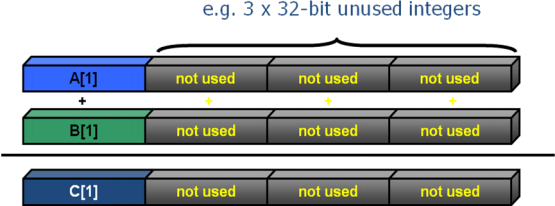
\includegraphics[width=\textwidth]{Registers_Unused.png}
      \caption{Disabled vectorization.}
      \label{fig:a}
    \end{minipage}
    \hspace{0.5cm}
    \begin{minipage}[b]{0.465\linewidth}
      \centering
      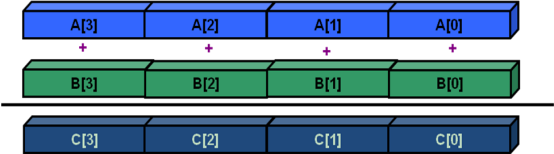
\includegraphics[width=\textwidth]{Registers_Used.png}
      \caption{Enabled vectorization.}
      \label{fig:b}
    \end{minipage}
  \end{figure}
\end{frame}

\begin{frame}{Vectorization criteria}{Which loops can be vectorized?}
  \begin{description}
  \item[Countable] The loop trip count must be known at entry to the
    loop at runtime and must not be data-dependent.
  \item[Single entry and single exit] The loop must not contain break
    commands.
  \item[Straight-line code] Branches are permitted only if they can be
    implemented as masked assignments.
  \item[The innermost loop of a nest] Only the innermost loop of nested
    loops can be vectorized, unless an outer loop is made the
    innermost loop by a different optimization method.
  \item[No function calls] The loop must not contain function calls,
    unless they are inline functions (in order to have straight-line
    code).
  \end{description}
\end{frame}

\begin{frame}[fragile]{Obstacles to vectorization}{Non-contiguous
    memory access}
  If the variables are not adjacent in memory, there is no point in
  vectorization as they can't be operated upon in a single
  instruction.
\begin{minted}{C}
// arrays accessed with stride 2
for (i = 0; i < SIZE; i += 2)
    b[i] += a[i] * x[i];

// inner loop accesses a with stride SIZE
for (j = 0; j < SIZE; j++) {
    for (i = 0; i < SIZE; i++)
        b[i] += a[i][j] * x[j];
}

// indirect addressing of x using index array
for (i = 0; i < SIZE; i++)
    b[i] += a[i] * x[index[i]];
\end{minted}
\end{frame}

\begin{frame}[fragile]{Obstacles to vectorization}{Data dependencies}
  Vectorization entails changes in the order of operations
  \(\implies\) there must not be any data dependencies.
\begin{minted}{C}
// read-after-write
A[0] = 0;
for (j = 1; j < MAX; j++)
    A[j] = A[j - 1] + 1;

// write-after-read
for (j = 1; j < MAX; j++)
    A[j - 1] = A[j] + 1;
\end{minted}
\end{frame}

\subsection{Automatic parallelization}

\begin{frame}{Automatic parallelization}
  \begin{itemize}
  \item Vectorization is useful when we perform a single operation on
    lots of data.
  \item However, some code cannot be vectorized, but can still be
    divided into independent chunks.
  \item These chunks can be run in parallel \(\implies\) have the
    compiler detect loops which can be parallelized.
  \end{itemize}
  This is a \emph{concurrent} approach.
\end{frame}

\begin{frame}{Parallelization criteria}{Which loops can be
    parallelized?}
  \begin{itemize}
  \item The number of iterations must be known before entry into a
    loop so that the work can be divided in advance (while loops
    cannot be done in parallel).
  \item There can be no jumps into or out of the loop.
  \item The loop iterations must be independent.
  \end{itemize}
\end{frame}

\section{Conclusion}

\begin{frame}{Conclusion}
  We presented and analyzed two recent topics in compilers and
  programming languages: dependent types and automatic parallelization
  and vectorization.

  \begin{itemize}
  \item Dependent types found their first uses in proof assistants
    such as
    \href{http://wiki.portal.chalmers.se/agda/pmwiki.php}{Agda} and
    \href{https://coq.inria.fr/}{Coq}.
  \item The \href{https://www.idris-lang.org/}{Idris} language uses
    dependent types for general-purpose programming.
  \item Automatic parallelization and vectorization are ``The Holy
    Grail'' of compiler optimizations.  However, they are currently
    limited to simple blocks of code, and many open problems remain.
  \end{itemize}
\end{frame}

\begin{frame}[allowframebreaks]{References}
  \printbibliography{}
\end{frame}

\end{document}

%%% Local Variables:
%%% mode: latex
%%% TeX-master: t
%%% TeX-engine: luatex
%%% TeX-command-extra-options: "-shell-escape"
%%% End:
